\chapter{Introduction}
\section{Research scope and motivation}


The domain of the proposed thesis is Automated Software Engineering. The thesis will develop methods for the analysis of legacy software systems, focusing on using historical information describing the evolution of the systems extracted from the versioning systems. 
The methods for analysis will integrate techniques based on computational algorithms as well as data-mining. As proof-of-concept, tool prototypes will implement the proposed methods and validate them by extensive experimentation on several cases of real-life systems.\\

\section{Objectives of the thesis}



\section{Structure of the thesis}

\section{Main Contributions}



%%%%%%%%%%%%%%%%%%%%%%%%%%%%%%%%%%%%%%%%%%%%%%%%%%%%%

\chapter{Software Dependencies: concepts, applications, and current research}
\label{dep}

\section{Software dependencies overview}

\subsection{Structural dependencies}
\hspace{4em} A dependency is created by two elements that are in a relationship and indicates that an element of the relationship, in some manner, depends on the other element of the relationship \cite{Booch:2004:OAD:975416}, \cite{Cataldo2009SoftwareDW}.

Structural dependencies can be found by analyzing the source code \cite{Sangal:2005:UDM:1094811.1094824}, \cite{CalloArias2011}. 
There are several types of relationships between these source code entities and all those create \textit{structural dependencies}:

\textbf{Data Item Dependencies.}
Data items can be variables, records or structures. A dependency is created between two data items when the value held in the first data item is used or affects the value from the second.


\begin{verbatim}
Example:

int a = 10;
int b = a + 5;  // b depends on a
a = 20;         // changing a doesn't impact b
\end{verbatim}

\textbf{Data Type Dependencies.}
Data items are declared to be of a specific data type. Besides the built-in data types that every programming language has, developers can also create new types that they can use. Each time the data type definition is changed it will affect all the data items that are declared to be of that type. 


\begin{verbatim}
Example:

class Rectangle { int width, height; }
//Change posibility: class Rectangle { int width, height, color; }

Rectangle r = new Rectangle();  
r.width = 5;
r.height = 10;
// Existing code will fail to handle color in case of change
\end{verbatim}

\textbf{Subprogram Dependencies.}
A subprogram is a sequence of instructions that performs a certain task. Depending on the programming language a subprogram may also be called a routine, a method, a function or a procedure. When a subprogram is changed, the developer must check the effects of that change in all the places that are calling that subprogram. Subprograms may also have dependencies with the data items that they receive as input or the data items that they are computing.


\begin{verbatim}
Example:

// First implementation:
class Calculator {
    double calculateArea(double side) {
        return side * side;  
    }
}

// Modified implementation:
class Calculator {
    double calculateArea(double radius) {
        return Math.PI * radius * radius; 
    }
}

Calculator calc = new Calculator();
// Code expecting square area now gets circle area.
double area = calc.calculateArea(5);  

\end{verbatim}





\subsection{Lexical dependencies}

\hspace{4em}Lexical dependencies, similar to structural dependencies, are extracted from the source code. The difference lies in the fact that lexical dependencies focus on finding pairs of entities that are similar (and thus connected) from a linguistic point of view. This means they are based on the textual content and naming conventions used in the code rather than explicit structural relationships. The lexical information about an entity (such as a class or interface) can be extracted from class names, method names, parameter names, code comments, source code statements, and others \cite{lexical-dep}, \cite{lexical-dep-Prajapati}.

For example, a class named \texttt{StructuralDependenciesEvaluator} and a class named \texttt{LexicalDependenciesEvaluation} can be related even if they do not directly share dependencies or their connection is not visible from a structural point of view.

To extract lexical dependencies, the code is tokenized, breaking it down into lexical tokens (e.g., words or symbols). A document containing these tokens is created for each source code file. Each document is then split into different parts, such as a class names part, attribute names part, parameter names part, and others. For instance, the class names part will contain the names of all classes found in the source file.

After the tokenization process and splitting into various parts, the similarity between the two documents is estimated. 

Various methods can be used for similarity calculation, such as:
\begin{itemize}
    \item \textit{Term Frequency-Inverse Document Frequency (TF-IDF):} Weighs the importance of words based on their frequency across documents \cite{lexical-dep}, \cite{lexical-dep-Corazza}.
    \item \textit{Cosine Similarity:} Measures the cosine of the angle between two vectors representing the documents \cite{lexical-dep-Prajapati}.
\end{itemize}






\subsection{Semantical dependencies}

\hspace{4em} Podgurski and Clarke define semantic dependencies in source code as follows: if changes in a statement \(s_1\) impact the behavior of another statement \(s_2\), then \(s_1\) and \(s_2\) are \emph{semantically dependent} \cite{Podgurski-semantic}.

Semantic dependencies can be identified from the source code by constructing control flow graphs (CFGs). A control flow graph is a directed graph \(G = (V, E)\), where:
\begin{itemize}
    \item \(V\) is the set of vertices representing program statements (e.g., assignments, method calls, conditions),
    \item \(E\) is the set of edges representing possible transfers of control between statements.
\end{itemize}

A vertex \(u \in V\) is semantically dependent on a vertex \(v \in V\) if changes in \(v\) determine changes in \(u\).

In object-oriented (OO) systems, semantic dependencies are dependencies that are not visible in the static structure of the code. There is no direct reference between two entities (e.g., classes or interfaces), but changes in one entity impact the behavior of the other \cite{Neto-semantic-dep}, \cite{Capiluppi-semantic-dep}.


\textit{Example:}

Let \(A\) a class that uses an object of type \(I\), and let \(B\) a class that implements \(I\). For example, class \(A\) calls a method \texttt{performAction()} via an interface \(I\), while class \(B\) implements the \texttt{performAction()} method.

If \(B\) changes its implementation of \texttt{performAction()}, the behavior of \(A\) might also change when it uses \(B\). This means that \(A\) and \(B\) are semantically dependent.






\subsection{Logical dedependencies}
\hspace{4em} \textit{Logical dependencies} (also known as logical coupling) can be discovered through software history analysis. They reveal relationships between entities that are not always present in the source code's static structure (i.e., structural dependencies).

Software engineering practice has shown that sometimes modules without explicit structural dependencies still appear to be related. \textit{Co-evolution} represents the phenomenon where one component changes in response to changes in another component \cite{Yu:2007:UCC:1231330.1231370, 5166450}. Such changes can be found in the software history maintained by version control systems. Gall et al. defined \textit{logical coupling} as the occurrence of modules that \emph{repeatedly} update together during the evolution of the software system \cite{Gall:1998:DLC:850947.853338, Gall:2003:CRH:942803.943741, 6606615}.

The concepts of logical coupling and logical dependencies have been applied in different analysis tasks related to software changes: for software change impact analysis \cite{1553643}; for identifying potential ripple effects caused by software changes during maintenance and evolution \cite{DBLP:conf/issre/OlivaG15, Oliva:2011:ISL:2067853.2068086, Poshyvanyk2009, posh2010}; and for exploring their link to defects \cite{wiese, Zimmermann:2004:MVH:998675.999460}.

An in-depth analysis of how logical dependencies are identified within the versioning system and their applications is provided in Section \ref{ld-intro}.






\subsection{Additional dependencies}

\hspace{4em} Besides the dependencies mentioned above, there are many other types of dependencies, such as temporal, package, external, and several others.

\textit{Temporal dependencies} represent a type of dependency where certain operations in the code must occur in a specific order. These operations may belong to the same software component or span across different parts of the system \cite{work-dep}.

\begin{verbatim}
Example:

var file = new File();
file.open("example.txt");
file.readContents();
file.close();
\end{verbatim}

In this example, there is a temporal dependency between the \texttt{open}, \texttt{readContents}, and \texttt{close} methods. The \texttt{readContents} method cannot function correctly unless the \texttt{open} method is called first to open the file. Similarly, the \texttt{close} method should be called after \texttt{readContents} to release the file resources.


\textit{Package dependencies} refer to the relationships between different software packages, usually managed using package managers \cite{dep-package}.

\textit{External dependencies} are the relationships between a software system's code and components outside the system, such as third-party services, libraries, APIs, or the programming language itself \cite{dep-external}.






\section{Software change and version control systems}

\subsection{Software change}
\label{change}

\hspace{4em} Software systems have distinctive stages during their life: initial development, evolution, servicing, phase out, and close down \cite{Software-life-cycle}, \cite{model-bennett}.

In the \textit{evolution stage}, iterative changes are made. By changes, we mean additions (new software features), modifications (changes of requirements or misunderstood requirements), or deletions. There are two main reasons for the change: the software team's learning process and new requests from the client.

Suppose new changes are no longer easy to be made or are very difficult and time-consuming. In that case, the software enters the \textit{servicing stage}, also called aging software, decayed software, and legacy \cite{Software-life-cycle}, \cite{363157}.

The main difference between changes made in the evolution and servicing stages is the effort to make changes. In the evolution stage, software changes are made easily and do not require much effort, while in the servicing stage, only a limited number of changes are made and require a lot of effort, so they are time-consuming \cite{Bennett}, \cite{Rajlich}.

The change mini-cycle consists of the following phases \cite{810308}:
\begin{itemize}
\item Phase 1: The change request. This usually comes from the software users, and it can also be a bug report or a request for additional functionality.
\item Phase 2: The planning phase includes program comprehension and change impact analysis. Program comprehension is a mandatory prerequisite of the change, while change
impact analysis indicates how costly the change will be. \cite{Bohner}
\item Phase 3: The change implementation, restructuring for change, and change propagation.
\item Phase 4: Verification and validation.
\item Phase 5: Re-documentation.
\end{itemize}

Understanding these phases is important for ensuring the software system remains maintainable and reliable throughout its lifecycle.


\subsection{Version control systems}

Software evolution implies change which can be triggered either by new feature requests or bug reports \cite{articleEvolution}. As presented also in section \ref{change}, one phase of the change mini-cycle consists of change implementation and propagation (changing source code files). 
Usually, developers use version control when it comes to software development. Version control is a system that records changes to a file or set of files over time so that developers can recall specific versions of those files later \cite{svn}.
Distributed version control systems (such as Git, Mercurial, Bazaar or Darcs) allows many developers to collaboratively develop their projects \cite{7471284}.

Below, we will review some of the operations supported by versioning systems. The operation names in the following text are specific to Git, as Git is the version control system used for data collection in the current work. However, similar operations exist in other versioning systems; for example, Subversion (SVN) and Mercurial also provide operations such as branching, merging, and committing changes.

\textbf{Repository}

A repository serves as a centralized storage location for project files. The entire codebase of a project can be stored within a single repository or be split into a main repository and various modules stored in multiple repositories. Git repositories can be hosted on numerous platforms, such as GitHub, GitLab, Bitbucket, and others.

It is important to differentiate between Git and Git hosting services. Git is a version control system that allows developers to download and modify code on their local devices while hosting services like GitHub provide platforms for teams to host projects that utilize Git \cite{git}, \cite{github}.

\textbf{Commits}

Committing is an operation that allows developers to record the latest changes to the codebase in the repository. A commit saves the current state of the code, including changes made since the last commit.

The changes tracked include:

\begin{itemize}
\item \textit{Additions:} New files or lines of code created.
\item \textit{Modifications:} Updates to existing lines of code or files.
\item \textit{Deletions:} Removal of files or lines of code that are no longer needed.
\end{itemize}

The \textit{push} operation uploads these changes to the remote repository on the hosting service.

A unique identifier, also known as a commit hash, is assigned to each commit. This hash allows developers to track specific changes or revert to earlier code versions. When a developer commits the changes, a commit message is required. This message serves as documentation for the changes, enhancing code traceability and maintainability \cite{git}.

Figure~\ref{fig:gitflow} illustrates how changes are made to the code over time through commits, starting from the initial commit to the latest version.

\begin{figure}[h!]
\centering
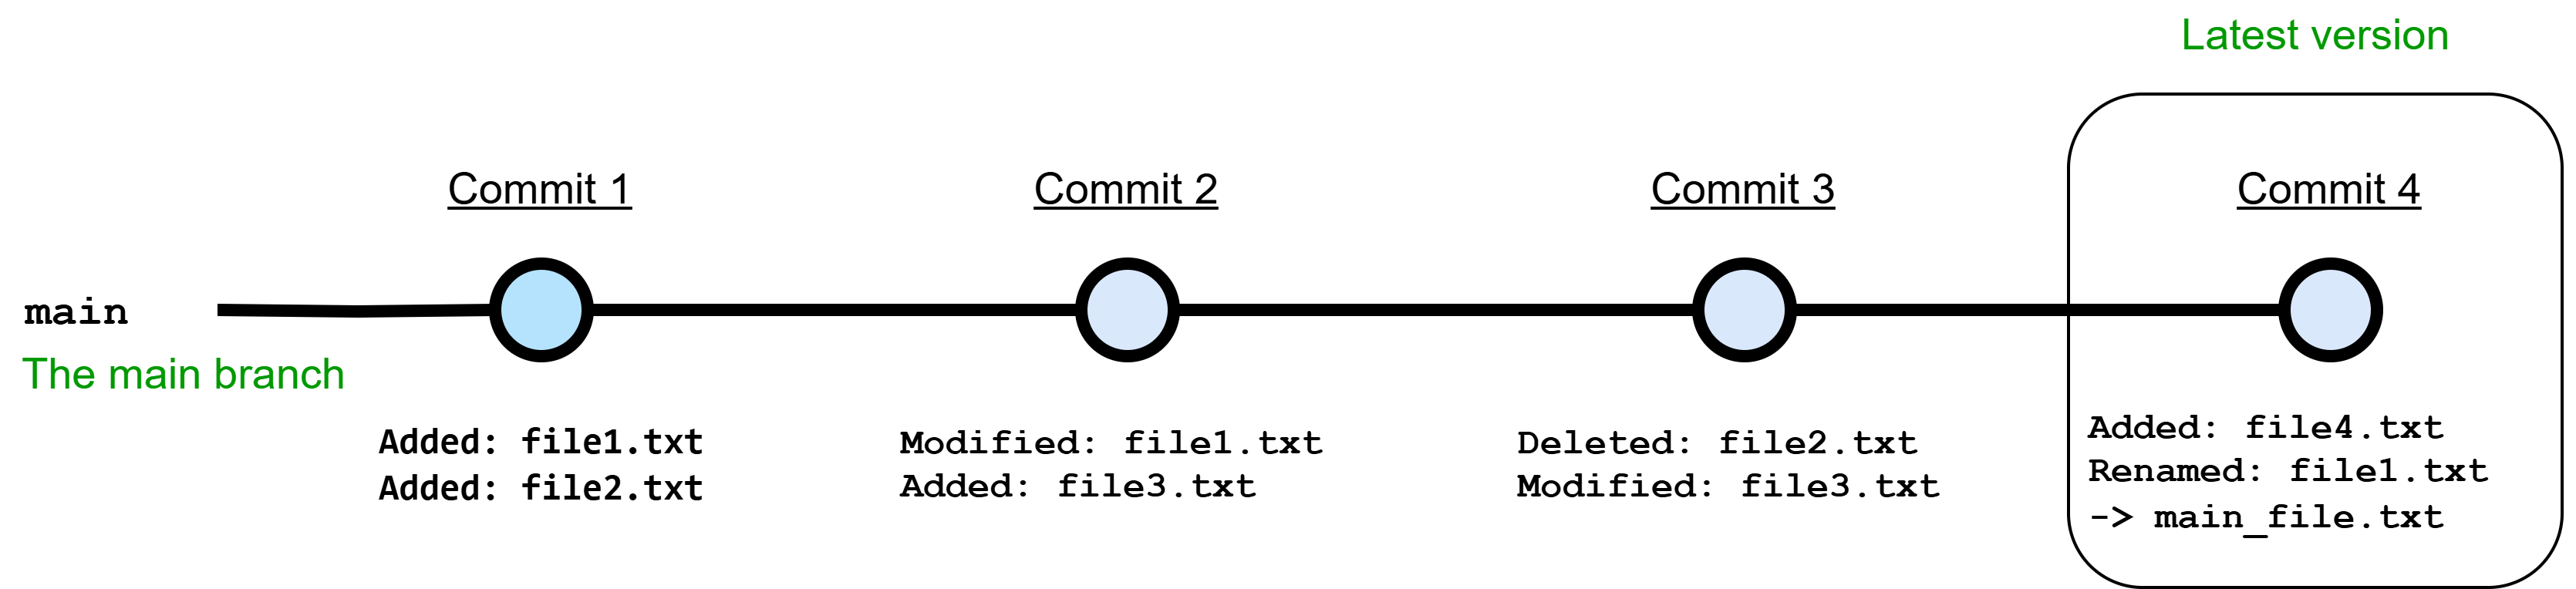
\includegraphics[width=\textwidth]{gitflow.png}
\caption{Tracking changes through commits.}
\label{fig:gitflow}
\end{figure}

\textbf{Branches and Merging}

By default, every repository comes with a main (or master) branch. This branch represents the central timeline for code changes and serves as the main integration point for stable code. Other branches can be created for parallel development from this branch.

Branches allow developers to encapsulate changes without affecting the main branch. In most software projects, it is standard practice for developers to use branches for development, with the main branch being locked for direct commits. Changes to the main branch can be integrated through merges from other branches.

Software projects often have multiple branches running in parallel, including branches from other branches. The main branch is not the only branch that supports branching; any branch can be a base for creating other branches.

The operation of integrating changes from one branch into another (usually into the main branch) is called \textit{merging}.

There are three main types of merges in Git \cite{git}:

\begin{itemize}
    \item \textit{Git Merge:} This is the most commonly used type of merging. It creates a new merge commit that combines all the changes from the branch being merged. Additionally, it retains the history of all the individual commits in the branch.
    \begin{verbatim}
    git checkout main
    git merge feature-branch
    \end{verbatim}

    \item \textit{Git Rebase and Merge:} This operation is typically used when the branch contains a single commit or a small number of commits. It moves all the commits from the source branch to the top of the target branch. The main disadvantage of this operation is that it rewrites the commit history.
    \begin{verbatim}
    git checkout feature-branch
    git rebase main
    git checkout main
    git merge feature-branch
    \end{verbatim}

    \item \textit{Git Squash and Merge:} This operation compresses all commits from the source branch into a single commit before merging it into the target branch. It results in a cleaner commit history but has the disadvantage of losing individual commits from the source branch.
    \begin{verbatim}
    git checkout main
    git merge --squash feature-branch
    git commit
    \end{verbatim}
\end{itemize}


Figure~\ref{fig:merging} illustrates the differences between these three types of merging. 

\begin{figure}[h!]
    \centering
    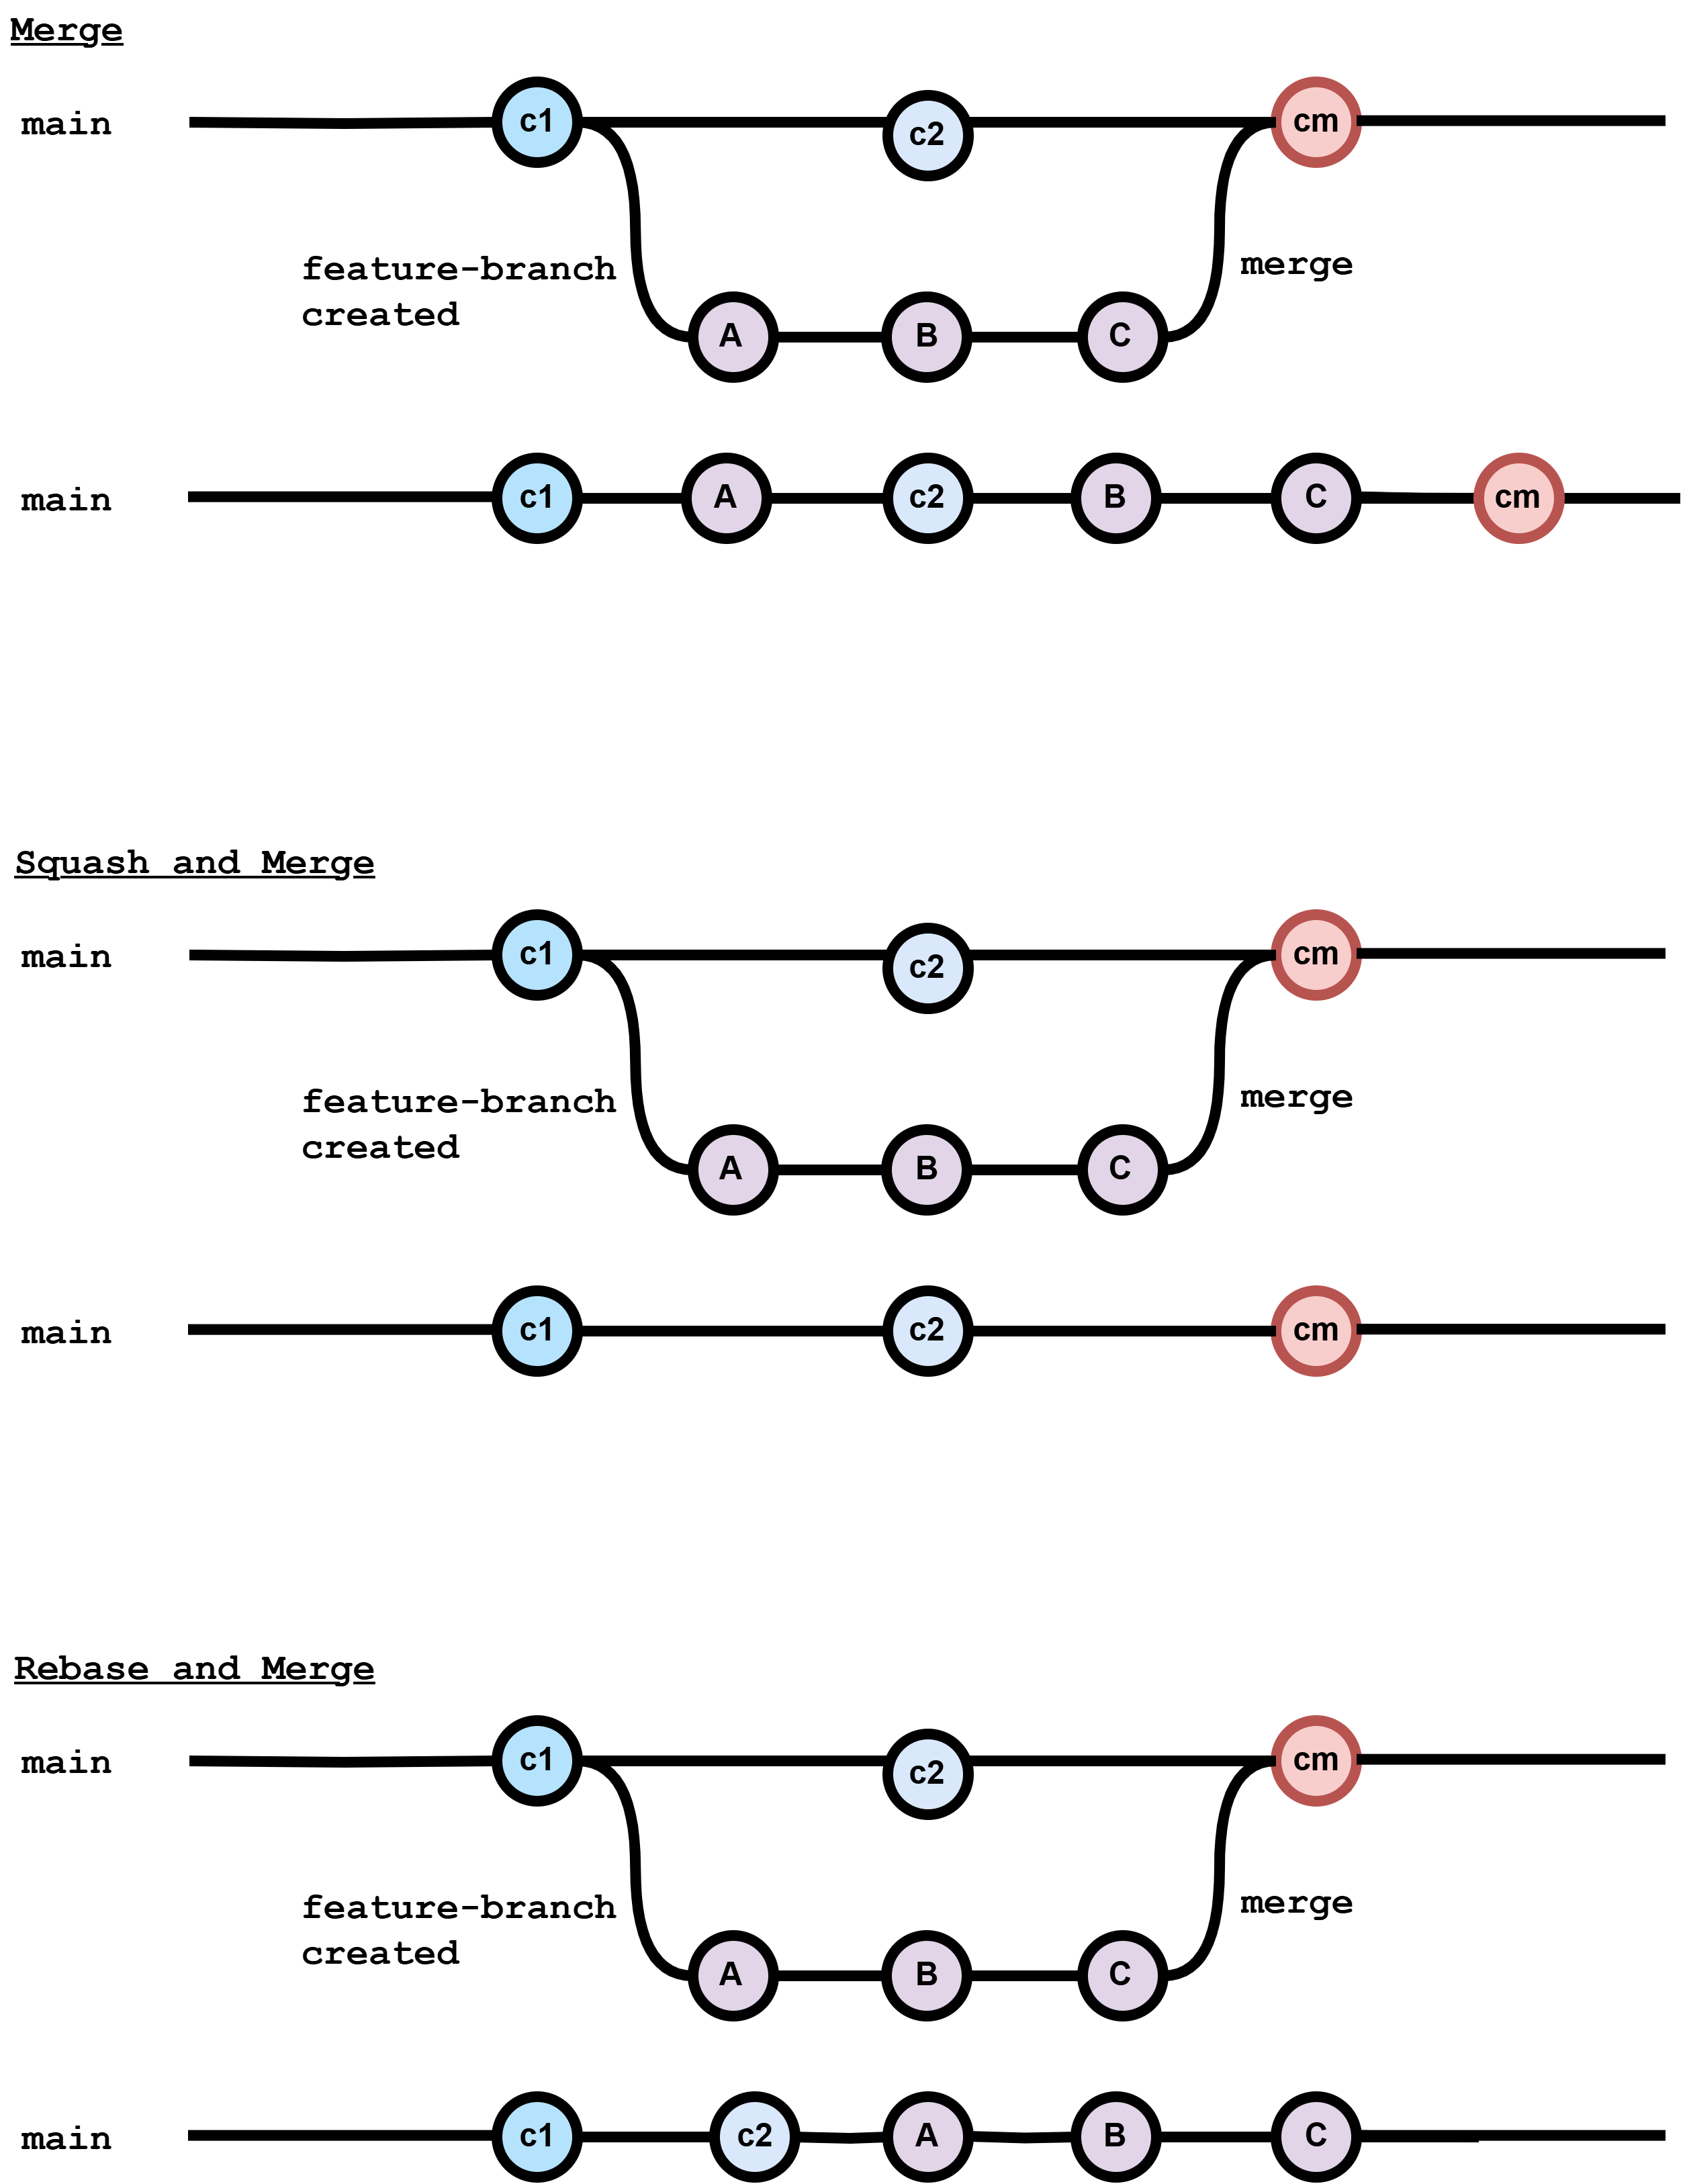
\includegraphics[width=\textwidth]{merging.png}
    \caption{Comparison of Git merge types.}
    \label{fig:merging}
\end{figure}

\textbf{Tagging}

Another helpful operation in Git is tagging. Developers use the tagging operation to mark a specific code version at a particular commit. This is usually done for important milestones, such as a new release version or a stable build \cite{git}.

Tags provide a way to create a human-readable reference to a specific commit (e.g., \texttt{v1.0.0}), as the commit hash can be hard to remember (e.g., \texttt{a1b2c3d4e5f6g7h8i9})

Git supports two types of tags:
\begin{itemize}
    \item \textit{Lightweight Tags:} Simple references to a commit that do not contain any additional metadata.
    \item \textit{Annotated Tags:} These include additional metadata such as the author's name, date, and message, making them more suited for marking releases.
\end{itemize}



\section{Current status of research on logical dependencies}
\label{ld-intro}

\subsection{Logical dependencies in software systems}

Oliva and Gerosa \cite{Oliva:2011:ISL:2067853.2068086}, \cite{DBLP:conf/issre/OlivaG15} have found first that the set of co-changed classes was much larger compared to the set of structurally coupled classes. They identified structural and logical dependencies from 150000 revisions from the Apache Software Foundation SVN repository. Also they concluded  that in at least 91\% of the cases, logical dependencies involve files that are not structurally related. This implies that not all of the change dependencies are related to structural dependencies and there could be other reasons for software artifacts to be change dependent.

Ajienka and Capiluppi also studied the interplay between logical and structural coupling of software classes. In \cite{DBLP:journals/jss/AjienkaC17} they  perform experiments on 79 open source systems: for each system, they determine the sets of structural dependencies, the set of logical dependencies and the intersections of these sets. They quantify the overlapping or intersection of these sets, coming to the conclusion that not all co-changed class pairs (classes with logical dependencies) are also linked by structural dependencies. One other interesting aspect which has not been investigated by the authors in \cite{DBLP:journals/jss/AjienkaC17}  is the total number of logical dependencies, reported to the total number of structural dependencies of a software systems. However, they provide the raw data of their measurements and we calculated the ratio between the number of logical dependencies and the number of structural dependencies for all the projects analyzed by them: the average ratio resulted 12.  This means that, using their method of detecting logical dependencies for a system, the number of logical dependencies outnumbers by one order of magnitude the number of structural dependencies. We consider that such a big number of logical dependencies needs additional filtering. 


Another kind of non-structural dependencies are the semantic or conceptual dependencies \cite{Poshyvanyk2009}, \cite{posh2010}. Semantic coupling is given by the degree to which the identifiers and comments from different classes are similar to each other. Semantic coupling could be an indicator for logical dependencies, as studied by Ajienka et al in \cite{DBLP:journals/ese/AjienkaCC18}. The experiments showed that a large number of co-evolving classes do not present semantic coupling, adding to the earlier research which showed that a large number of co-evolving classes do not present structural coupling. All these experimental findings rise the question whether it is a legitimate approach to accept all co-evolving classes as logical coupling.

Zimmermann et al \cite{Zimmermann:2004:MVH:998675.999460} introduced data mining techniques to obtain association rules from version histories.
The mined association rules  have a probabilistic interpretation based on the amount of evidence in the transactions they are derived from. This amount of evidence is determined by two measures: support and confidence.  They developed a tool to predict future or missing changes.

Different applications based on dependency analysis could be improved if, beyond structural dependencies, they also take into account the hidden non-structural dependencies. For example, works  which investigate different methods for architectural reconstruction \cite{SoraConti}, \cite{SoraSem13}, \cite{PagerankENASE},  all of them based on the information provided by structural dependencies, could enrich their dependency models by taking into account also logical dependencies. However, a thorough survey \cite{sar} shows that historical information has been rarely used in architectural reconstruction. 

Another survey \cite{Shtern:2012:CMS:2332427.2332428} mentions one possible explanation why historical information have been rarely used in architectural reconstruction: the size of the extracted information. One problem is the size of the extraction process, which has to analyze many versions from the historical evolution of the system. Another problem is the big number of pairs of classes which record co-changes and how they relate to the number of pairs of classes with structural dependencies.

The software architecture is important in order to understand and maintain a system. Often code updates are made without checking or updating the architecture. This kind of updates cause the architecture to drift from the reality of the code over time \cite{sar}.
So reconstructing the architecture and verifying if still matches the reality is important \cite{Kalliamvakou2016}. 

Surveys also show that architectural reconstruction is mainly made based on structural dependencies \cite{Shtern:2012:CMS:2332427.2332428}, \cite{sar}, the main reason why historical information is rarely used in architectural reconstruction is the size of the extracted information.

Logical dependencies should integrate harmoniously with structural dependencies in an unitary dependency model: valid logical dependencies should not be omitted from the dependency model, but structural dependencies should not be engulfed by questionable logical dependencies generated by casual co-changes.  
Thus, in order to add logical dependencies besides structural dependencies in dependency models, class co-changes must be filtered until they remain only a reduced but relevant set of valid logical dependencies. 

Currently there is no set of rules or best practices that can be applied to the extracted class co-changes and can guarantee their filtering into a set of valid logical dependencies.
This is mainly because not all the updates made in the versioning system are code related. For example a commit that has as participants a big number of files can indicate that a merge with another branch or a folder renaming has been made. In this case, a series of irrelevant co-changing pairs of entities can be introduced. So, in order to exclude this kind of situations the information extracted from the versioning system has to be filtered first and then used.

Other works have tried to filter co-changes \cite{Oliva:2011:ISL:2067853.2068086}, \cite{DBLP:journals/jss/AjienkaC17}. One of the used co-changes filter is the commit size.The commit size is the number of code files changed in that particular commit. 
Ajienka and Capiluppi established a threshold of 10 for the maximum accepted size for a commit \cite{DBLP:journals/jss/AjienkaC17}. This means that all the commits that had more than 10 code files changed where discarded from the research. But setting a harcoded threshold for the commit size is debatable because in order to say that a commit is big or small you have to look first at the size of the system and at the trends from the versioning system. Even thought the best practices encourage small and often commits, the developers culture is the one that influences the most the trending size of commits from one system.

Filtering only after commit size is not enough, this type of filtering can indeed have an impact on the total number of extracted co-changes, but will only shrink the number of co-changes extracted without actually guaranteeing that the remaining ones have more relevancy and are more logical linked.

Although, some unrelated files can be updated by human error in small commits, for example: one file was forgot to be commited in the current commit and will be commited in the next one among some unrelated files. This kind of situation can introduce a set of co-changing pairs that are definitely not logical liked. In order to avoid this kind of situation a filter for the occurrence rate of co-changing pairs must be introduced. Co-changing pairs that occur multiple times are more prone to be logically dependent than the ones that occur only once. Currently there are no concrete examples of how the threshold for this type of filter can be calculated. In order to do that, incrementing the threshold by a certain step will be the start and then studying the impact on the remaining co-changing pairs for different systems. 

Taking into account also structural dependencies from all the revisions of the system was not made in previous works, this step is important in order to filter out the old, out-of-date logical dependencies. Some logical dependencies may have been also structural in previous revisions of the system but not in the current one. If we take into consideration also structural dependencies from previous revisions then the overlapping rate between logical and structural dependencies could probably increase. Another way to investigate this problem could be to study the trend of concurrences of co-changes: if co-changes between a pair of classes used to happen more often in the remote past than in the more recent past, it may be a sign that the problem causing the logical coupling has been removed in the mean time. 

\subsection{Existing filtering techniques}
tbd


\section{Applications of software dependencies}
\label{app}

\subsection{Reverse engineering}
The term reverse engineering was first defined by Chikofsky and Cross \cite{ChikofskyReverse} as the \textit{"process of analyzing a system to (i) identify the system’s components and
their inter-relationships and (ii) create representations of the system in another form or at a higher level of abstraction."} 

Reverse engineering is viewed as a two step process: information extraction and abstraction. \cite{FoSEReverseEngineering} 
The firs step, information extraction, is made by source code analysis which generates dependencies between software artifacts. So, reverse engineering uses dependencies in order to create new representations of the system or provide a higher level of abstraction \cite{struct_dep}, \cite{Gueheneuc}.

\subsection{Architecture reconstruction}
Currently, the software systems contain tens of thousands of lines of code and are updated multiple times a day by multiple developers.  
The software architecture is important in order to understand and maintain a system. Often code updates are made without checking or updating the architecture.
This kind of updates cause the architecture to drift from the reality of the code over time. So reconstructing the architecture and verifying if still matches the reality is important. \cite{sar},\cite{PagerankENASE}, \cite{Bass-archreconstruction} ,\cite{RecoverySartipi}, \cite{model-bennett}.

\subsection{Identifying clones}
Research suggests that a considerable part (around 5-10\%) of the source code of large-scale software is duplicate code (“clones”). Source code is often duplicated for a variety of reasons, programmers may simply be reusing a piece of code by copy and paste or they may be “reinventing the wheel” \cite{ClonesMayrand}, \cite{clones}.
Detection and removal of clones can decrease software maintenance costs \cite{CloneDetection}, \cite{cloneKamiya}.

\subsection{Code smells }
Code smells have been defined by Fowler \cite{bookFowler} and describe patterns that are generally associated with bad design and bad programming practices.
Originally, code smells are used to find the places in software may need refactoring \cite{articlesmells}. Studies have found that smells may affect comprehension and possibly increase change and fault proneness \cite{5741260}, \cite{5328703}, \cite{articlefault-proneness}.
Examples of code smells:
\begin{itemize}
	\item Large Class: one class with many fields.
	\item Feature Envy:  methods that access more methods and fields of another class than of its own class.
	\item Data Class: classes that only fields and do not contain functionality.
	\item Refused Bequest: classes that leave many of the fields and methods they inherit unused
	\item Parallel Inheritance: every time you make a subclass of one class you also have to make a subclass of the other.
	\item Shotgun Surgery: one method is changing together with other methods contained other classes.
\end{itemize}

Previous studies already explored the idea of using history information in order to detect code smells \cite{6963448}. 

\subsection{Comprehension}
Software comprehension is the process of gaining knowledge about a software system.
An increased knowledge of the software system help activities such as bug correction, enhancement, reuse and documentation \cite{Comprehension}, \cite{1199197}, \cite{2003:XLC:851042.857028}.
Previous studies show that the proportion of resources and time allocated to maintenance may vary from 50\% to 75\% \cite{articleLientz}.
Regarding maintenance, the greatest part of the software maintenance process is the activity of understanding the
system. 
Thanking into consideration the previous statements we can say that if we want to improve software maintenance we have to improve software comprehension \cite{article-cognitive-processes}.

\subsection{Fault location}
Debugging software is an expensive and mostly manual process. Of all debugging activities, fault localization, is the most expensive \cite{articleDebugging}. 

Software developers locate faults in their programs using a manual process. This process begins when the developers observe failures in the program. The developers choose a set of data to inject in the system(a set of data that most likely replicate previous failures or may generate new ones) and place breakpoints using a debugger. Then they observe the system's state until an failed state is reached, and then backtrack until the fault is found. 

As we said, this process has high costs so because of this high cost, any improvement in the process can decrease the cost of debugging.\cite{fault-localization} \cite{program-failures}


\subsection{Error proneness}
Research has shown that based on the software error history and simple metrics related to the amount of data and the structural complexity of software,
modules that are most likely to contain errors can be identified \cite{67595}, \cite{1702015}.


\subsection{Empirical software engineering research}
Empirical research tries to explore, describe, predict, and explain natural or social phenomena by using evidence based on observation or experience.
It involves obtaining and interpreting evidence by experimentation, systematic observation, interviews, surveys, or by the careful examination of documents and artifacts. \cite{inproceedingsEmpirical}
